\documentclass{beamer}
\usepackage[utf8x]{inputenc}
\usepackage{default}
\usepackage{graphics}
\usetheme{Luebeck}
\useinnertheme{rounded}
\usecolortheme{whale}
\graphicspath{{pics/}}


\usepackage{tikz}
\usetikzlibrary{arrows}
\tikzstyle{block}=[draw opacity=0.7,line width=1.4cm]

\usepackage{pgfpages}
\pgfpagesuselayout{2 on 1}[a4paper,border shrink=5mm]

\setbeameroption{show notes}
\setbeameroption{notes on second screen}
\setbeamertemplate{note page}[plain]
\setbeamertemplate{footline}[frame number]
\beamertemplatenavigationsymbolsempty

\title{Novelty Detection for Visual Place Classification}
\author{André Susano Pinto\inst{1}}

\institute[FEUP] {
 \inst{1}Faculdade de Engenharia da Universidade do Porto
}

\begin{document}
\begin{frame}
 \titlepage
\end{frame}

\begin{frame}{Outline}
 \tableofcontents
\end{frame}



\section{Introduction}

\subsection{Project}
\begin{frame}{Master Thesis}

\begin{block}{}
\textbf{Title}: Novelty Detection for Visual Place Classification

\textbf{Student}: André Susano Pinto (student at FEUP currently Erasmus in KTH).
\end{block}


\begin{columns}[t]
  \column{.5\textwidth}
  \begin{block}{}
    \textbf{Supervisor}: Luis Paulo Reis at FEUP
  \end{block}
  \column{0.5\textwidth}
  \begin{block}{}
    \textbf{Supervisor}: Andrzej Pronobis at CVAP (Computer Vision and Active Perception) in KTH
  \end{block}
\end{columns}

\note{
\begin{itemize}
\item Hi my name is André and at the moment I am studying in KTH in Stockholm as an exchange student (free mover).
\item My master thesis topic will be on "Novelty detection for Visual Place Classification".
\item And it will also be performed in KTH on the Computer Vision and Active Perception lab. My supervisor there will be Andrzej Pronobis.
\item And my supervisor in FEUP will be Luis Paulo Reis.
\end{itemize}
}

\end{frame}


\subsection{Motivation}
\begin{frame}{Motivation}
\begin{itemize}
\item A.I. and robotics focus in cognitive robots able to interact with humans and man-made environments.
\item The ability to classify the environment leads to reliable navigation but also in higher-level semantic space interpretation.
\item Novelty detection allows to distinguish between what is known and what is unknown.
\end{itemize}
%-And will allow the robot to detect surprise.

\note{
\begin{itemize}
\item There has been several efforts in the area of Robotics and Artifical Inteligence in creating robots that are able to interact with humans.
\item Those robots often have to navigate on indoor rooms such as kitchens, corridors and the ability for the robot to navigate in those is crucial.
\item A correct identification of the type of room also brings easier human interaction as a human would be able to say: "Bring me a tea cup from kitchen". And the robot should be smart enough to identify the kitchen.
\item Also crucial is the ability of the robot to operate on unknown environments as often the robot cannot be trained with the environment it will be deployed to.
\item In that context understanding the properties that represent a room category and be able deal with suprise and unknown becomes crucial too. Hence the importance of be able to detect novelty.
\end{itemize}
}
\end{frame}



\section{Problem Description}

\subsection{Robot Knowledge Layers}
\begin{frame}

\begin{columns}[t]
  \begin{column}{.5\textwidth}
    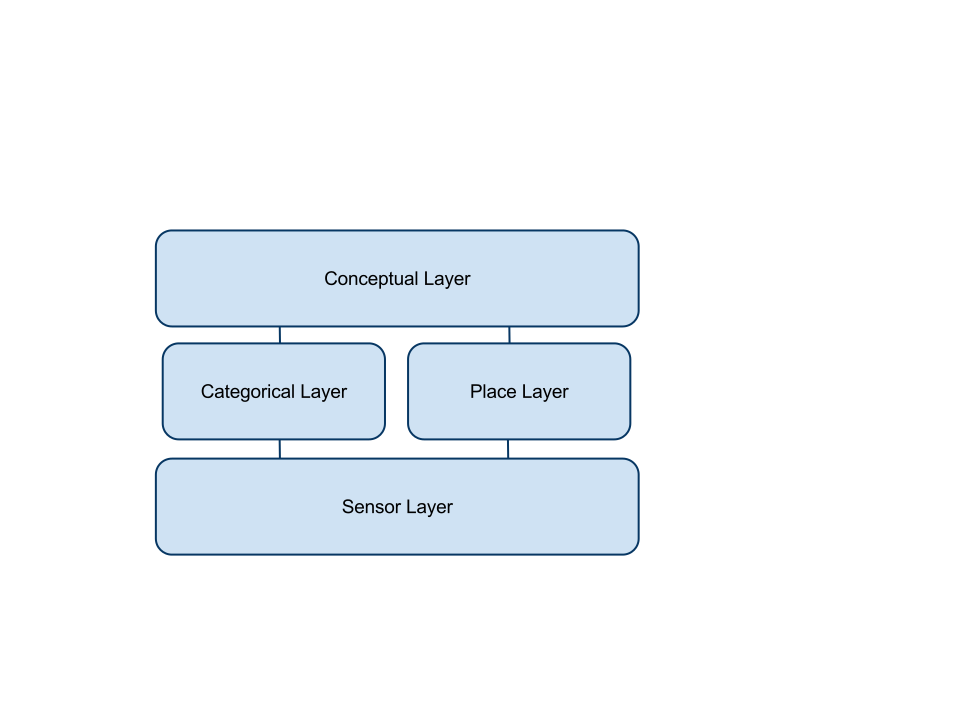
\includegraphics[width=.95\textwidth]{RobotLayers}
  \end{column}
%  \cite{spatial_knowledge}
  
%\begin{itemize}
%\item Sensorial
%\item Place
%\item Categorical
%item Conceptual Layer
%\end{itemize}

  \begin{column}{.5\textwidth}
	\includegraphics[width=.95\textwidth]{screenshot-0003}
  \end{column}

\end{columns}
\note{
I will now describe in more detail the robot architecture in which the problem is inserted on.

\begin{itemize}
\item As the robot navigates through the environment peforming SLAM (Simulataneous Localization and Mapping) its sensor laser captures data from the environ. That data is composed of scans, imagery from cameras and depth information.
\item From that data the robot extracts given properties for its current position. We can see on the image the robot classification of the rooms as square, elongated.
\item At the same time the robot creates a graph of its positions and estimates a distribution of those properties for each node.
\item Then at an higer level the robot performs classification of each room using the extracted properties and the knowledge it has from each class. In the picture we can see the robot classification for each type of room. For example it was able to detect the corridor.
\end{itemize}
}
\end{frame}

\subsection{Property based mapping}
\begin{frame}{Property based mapping}
A property mapping allows the system to explain how rooms are categorized.

\begin{block}{Example}
\begin{itemize}
 \item A corridor has elongated shape and is usually empty.
 \item A kitchen usually contains cereal boxes.
\end{itemize}
\end{block}

\note{
\begin{itemize}
\item It has been sugested that certain groups of features appear and disappear together between diferent room classses.
\item Those can be seen as set of features generated by some property of the room.
\item For example an elongated shape room or a room containing a cereal box will often triggerthe same subset of features.
\item Performing such a mapping is important for the problem in question as it greatly increase robot-human iteraction by allowing a robot to explain the properties that lead to decisions.
\end{itemize}
}
\end{frame}


\subsection{Place Classification with Novelty detection}
\begin{frame}
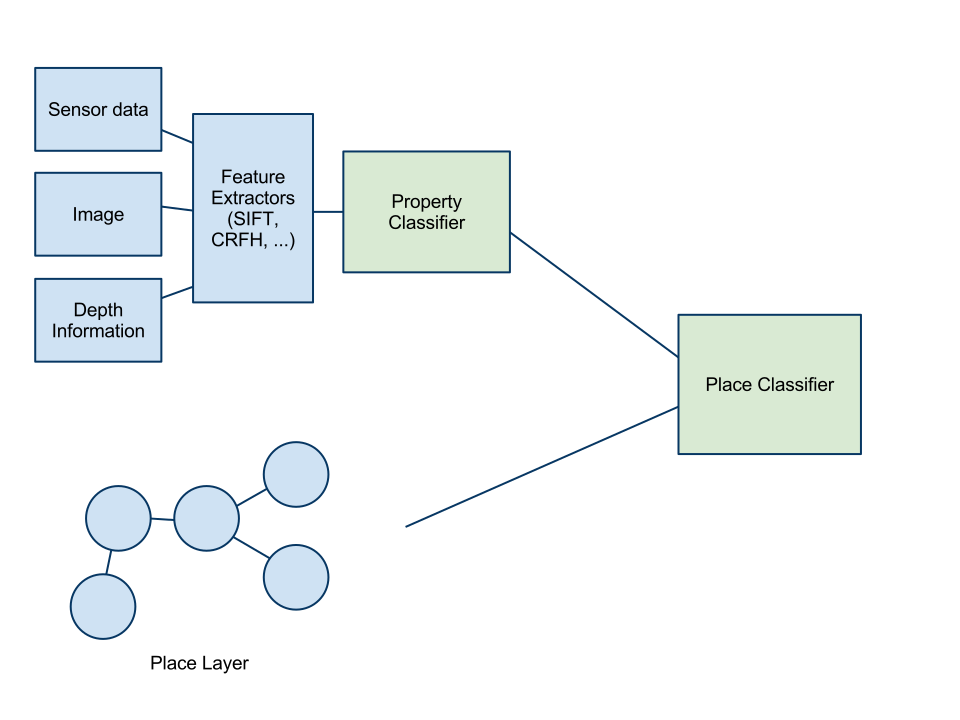
\includegraphics[width=0.95\textwidth]{NoveltyDetection}

\note{
With the give description on the plataform I can now explain where classification is performed.
\begin{itemize}
\item As said before the sensor layer will extract several feature descriptors from the input data.
\item Those features are then classified or well mapped to properties.
\item Then at a later stage those properties together with the place graph is used to classify the room.
\end{itemize}

So on the diagram those 2 classification parts are represented in green.
}

\end{frame}



\section{Solution Perspectives}

\begin{frame}{Solution - Place Classification}
\begin{block}{}
Given an input determine to which classe of a set C it is believed to be generated from.
\end{block}

\begin{itemize}
\item Usually performed by multiclass classifiers. Eg.: SVM (One-Against-All, One-againts-One).
\item High dimensional data leads to poor results as it fails to define a correct boundary over data.
\item Lacks ability to detect novel cases.
\end{itemize}

% \includegraphics<1>[width=0.5\textwidth]{place_classification}
\note{
\begin{itemize}
\item The problem of classification is one in which an algorithm has to assign an input into one of given categories.
\item It is often solved using several 2-class classifiers (for example Support Vector Machines).
\item Though it is know that for data with high dimension its becomes incredibly hard to define boundaries between the diferent classes.
\item Also those methods often lack ability to understand novel cases.
\end{itemize}
}
\end{frame}



\subsection{Novelty Detection}
% Used in methods where its hard to gather positive/negative sample of a class (eg.: Breast cancer, digit recognition)
\begin{frame}{Solution - Novelty Detection}
\begin{block}{}
Given an input determine if it was generated by the same class as the one seen before.
\end{block}

\begin{itemize}
\item Also known as Single Class Classifier.
\item Used when its hard or impossible to gather representative negative samples of a class (eg.: used on breast cancer detection).
\item Some of these methods are Kernel PCA and one-class SVMs.
\end{itemize}

\note{
\begin{itemize}
\item The solution passes then by implementing novelty detection methods, also known as single class classifiers.
\item Such a system task becomes then: given an input determine if it was generated by the same class as it was trained with.
\item And during my thesis diferent methods of performing novelty detection will be implemented and analised.
\item Such as Kernel PCA and one class-SVMs.
\end{itemize}
}

\end{frame}




\section{Technical Aspects}

\subsection{Databases and Test data}
\begin{frame}{Databases and Test data}

\begin{columns}[t]
\column{.5\textwidth}

\begin{block}{COsy Location Database}
\includegraphics[width=0.95\textwidth]{cold}
\end{block}

\column{.5\textwidth}

\begin{block}{ImageCLEF}
\includegraphics[width=1\textwidth]{imageclef-logo}
\end{block}

\end{columns}

\note{
\begin{itemize}
\item For training data databases such as COSY will be used. COsy is a database that contains imagery recorded from several labs.
\item It is also planned that the developed system will be partipate in the ImageCLEF competition.
\end{itemize}
}
\end{frame}




\section{Work Plan}
\begin{frame}{Work Plan}
\begin{itemize}
\item Literature Review (3 weeks)
\item Study of the property-base semantic mapping system (2 weeks)
\item Implementing novelty detection algorithms (3 weeks)
\item Implementing global and local features (3 weeks)
\item Testing and evaluating methods (5 weeks)
\item Thesis writting (4 weeks)
\end{itemize}
\end{frame}

\section{}
\begin{frame}{Thank You!}
 \titlepage

\end{frame}

\end{document}
